% Code listing configuration for MATLAB
\lstset{
    language=Matlab,
    basicstyle=\ttfamily\small,
    keywordstyle=\color{blue},
    stringstyle=\color{purple},
    commentstyle=\color{green!60!black},
    numbers=left,
    numberstyle=\tiny\color{gray},
    breaklines=true,
    frame=single,
    captionpos=b
}

\section{Exercise 8.15: The Fraunhofer diffraction pattern}
\subsection{MATLAB Implementation}

If the two-dimensional rectangular function represents an aperture with width $a$ and height $b$, its Fourier transform is the resulting Fraunhofer diffraction pattern. Given the function:
\begin{equation}
\label{eq:2DRect}
    f(x,y) = rect \left( \frac{x}{a} \right) rect \left( \frac{y}{b} \right)
\end{equation}

We can calculate the Fourier transform by computing the transform first with respect to one variable ($x$) and then with respect to the other ($y$).

\begin{equation}
    F(k_x,y) = a \cdot sinc \left( \frac{k_x a}{2} \right) rect \left( \frac{y}{b} \right)
\end{equation}

\begin{equation}
\label{eq:Fraunhofer}
    F(k_x,k_y) = a \cdot b \cdot sinc \left( \frac{k_x a}{2} \right) sinc \left( \frac{k_y b}{2} \right)
\end{equation}

We can compute these results in MATLAB by either having equation \ref{eq:2DRect} and using MATLAB's internal 2D fast Fourier transform method (fft2) or by graphing directly the analytical solution given by equation \ref{eq:Fraunhofer}. Both are done in the MATLAB code below.

NOTE: In MATLAB the sinc function is defined as: $sinc(u) = \frac{sin(\pi u)}{\pi u}$, therefore we must adjust this in the code for our analytical solution to match the numerical computation performed by MATLAB. 

\lstinputlisting[caption={MATLAB script \texttt{dft2\_rect.m}}, label={lst:dft2_rect}]{Code/dft2_rect.m}

\subsection{Results}

Plotted in figure \ref{fig:Fraunhofer} are the results of the analysis. There seems to be no difference between the analytical and numerical methods. Although if there is a lower resolution of the data, meaning N is lower, the differences are more noticeable. Figure \ref{fig:FraunhoferLowerQuality} shows the results of having N = 33.  

The main differences between the figure \ref{fig:FraunhoferLowerQuality}(b) and \ref{fig:FraunhoferLowerQuality}(c) are most visible along the outer lobes and null lines of the pattern, for example along the vertical wavenumber $k_y \approx 20$. \ref{fig:FraunhoferLowerQuality}(c) shows instantaneous 0 value where \ref{fig:FraunhoferLowerQuality}(b) has a more diffused line. This is due to aliasing, when the spatial sample size is reduced the aliasing effects are more noticeable in the discrete Fourier transform. In the case of the sinc function, with a lower Nyquist frequency aliasing is more noticeable in the result. 

\begin{figure} [H]
    \centering
    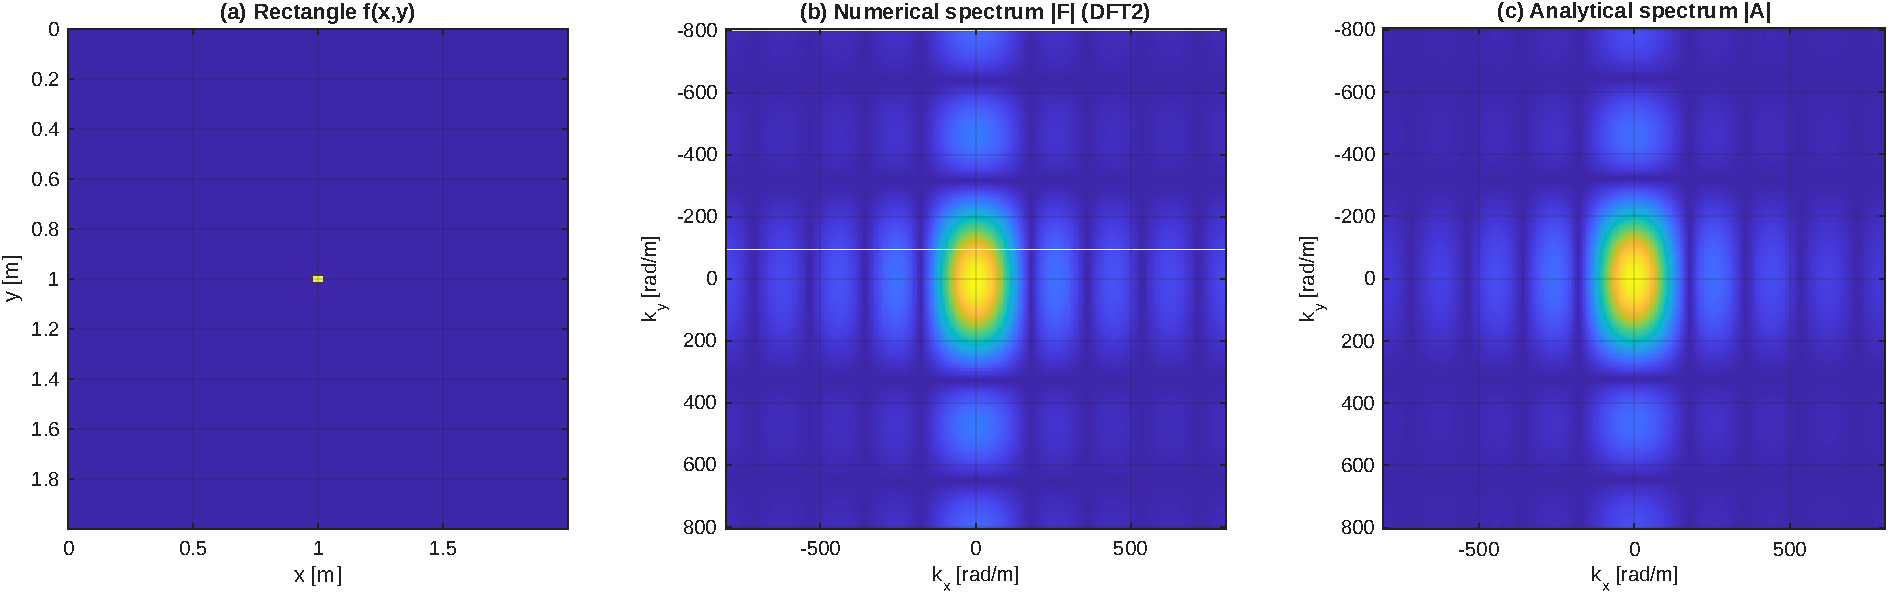
\includegraphics[width=1\linewidth]{Figures/Fraunhofer.pdf}
    \caption{Results of the MATLAB code. (a) window area. (b) numerical solution. (c) analytical solution.}
    \label{fig:Fraunhofer}
\end{figure}

\begin{figure} [H]
    \centering
    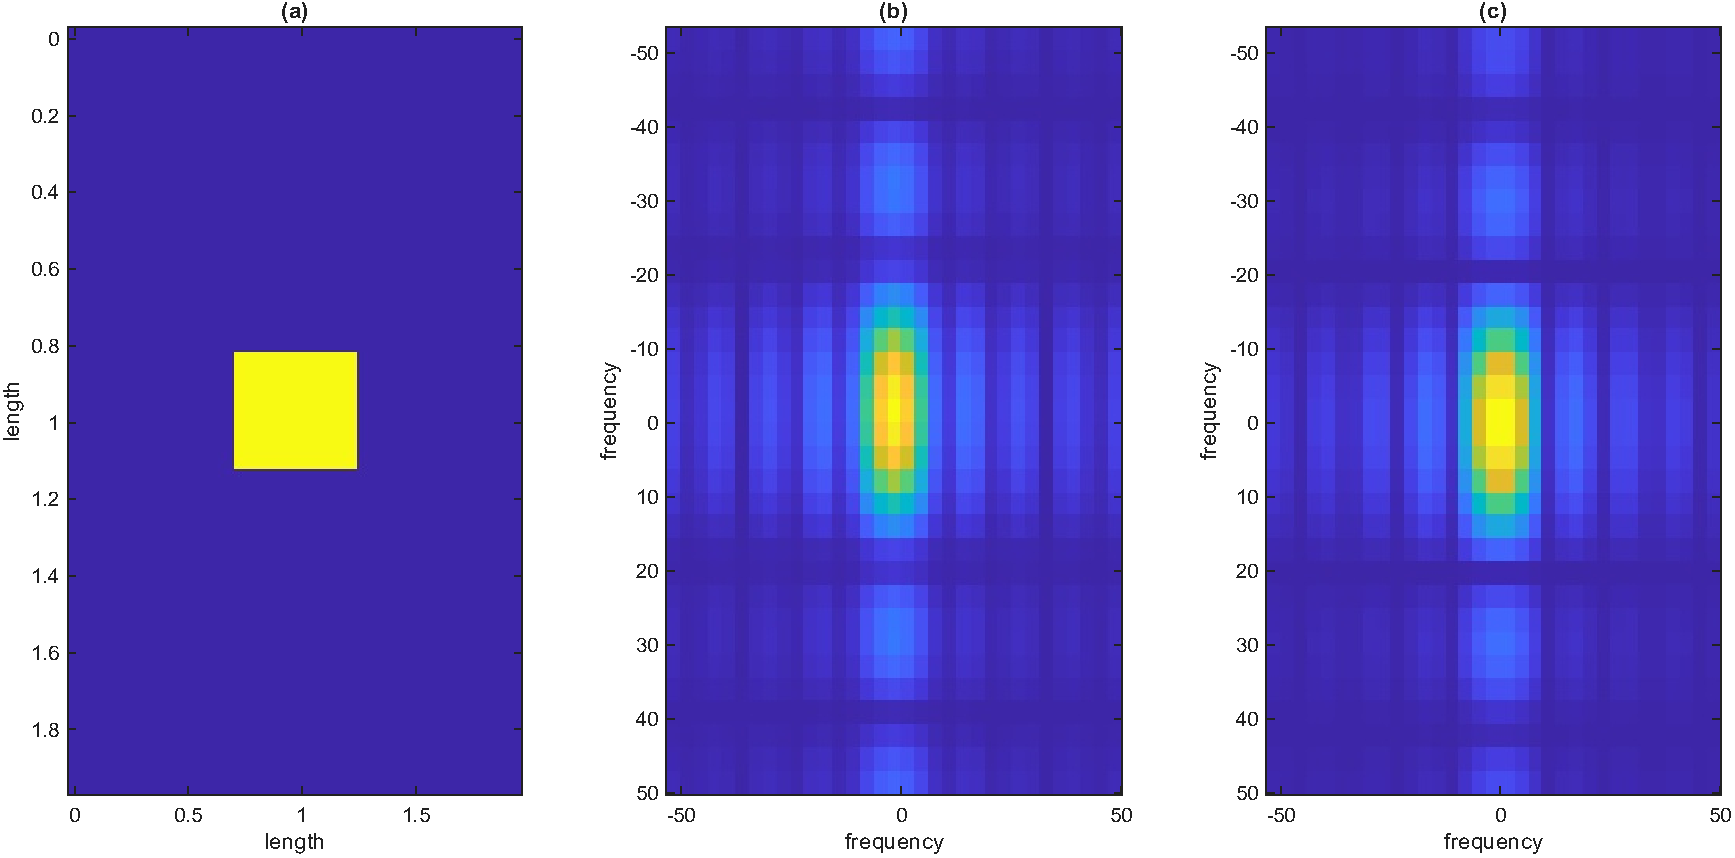
\includegraphics[width=1\linewidth]{Figures/FraunhoferLowerQuality.pdf}
    \caption{Results of the MATLAB code with N=33. (a) window area. (b) numerical solution. (c) analytical solution.}
    \label{fig:FraunhoferLowerQuality}
\end{figure}

